\label{sec:04TheResidualsanalysis}
\section{The Residuals $\varepsilon_t^2 = (X_t - X_{t-1})^2$ analysis}
\subsection{Plotting}
We will plot the residuals and residual squared of ARMA(1,0) series
\FloatBarrier
\begin{figure}[!htbp]
  \centering
  \includegraphics[width=\textwidth]{img/Fig8.eps}
  \caption{The Residual plot}
\end{figure}
\FloatBarrier
\FloatBarrier
\begin{figure}[!htbp]
  \centering
  \includegraphics[width=\textwidth]{img/Fig9.eps}
  \caption{The Residual Squared plot}
\end{figure}
\FloatBarrier
\subsection{Distribution Checking}
In order to check the distribution, we first run $shapiro.test()$ function, which will run the Shapiro-Wilk Test \cite{royston1982extension} with following results:
\begin{lstlisting}[language=R, caption=Shapiro-Wilk normality test]
Shapiro-Wilk normality test
data:  Resids
W = 0.98495, p-value = 2.991e-10
\end{lstlisting}
The $H_0$: Normal Distribution \\
The $H_1$: Not Normal Distribution \\
The p-value is less than 0.05, so we can concluded that the Residuals are not distributed Normality. 

\FloatBarrier
\begin{figure}[!htbp]
  \centering
  \includegraphics[width=\textwidth]{img/Fig10.eps}
  \caption{The Normal Distribution QQ plot of ARMA residuals}
\end{figure}
\FloatBarrier
Then we will test with Student's t-distribution with $ks.test.t()$ function - based on Kolmogorov-Smirnov test \cite{dujrbin1973distribution}, and received following outcome:
\begin{lstlisting}[language=R, caption=Kolmogorov-Smirnov test student-t with df=7.42]
data:  fit1$residuals
D = 0.015544, p-value = 0.9166
\end{lstlisting}
The $H_0$: Student's t-distribution \\
The $H_1$: Not Student's t-distribution \\
The p-value is higher than 0.05, so we can concluded that the Residuals are Student's t-distribution. 

\FloatBarrier
\begin{figure}[!htbp]
  \centering
  \includegraphics[width=\textwidth]{img/Fig11.eps}
  \caption{The Student's t-distribution QQ plot of ARMA residuals}
\end{figure}
\FloatBarrier

\subsection{Autocorrelation Test}
We use the Box-Ljung Test \cite{box1970distribution,ljung1978measure}, which indicated in $Box.test()$ function to test the Autocorrelation of Residuals as following:
\begin{lstlisting}[language=R, caption=Box-Ljung test]
Box-Ljung test
data:  fit1$residuals
X-squared = 73.912, df = 50, p-value = 0.01559
\end{lstlisting}
The $H_0$: The residuals are independently distributed \\
The $H_1$: The residuals are not independently distributed \\
p-value less than 0.05 then reject the Null Hypothesis, which means the residuals are independently distributed.\\
The below ACF and PACF plots also support this conclusion
\FloatBarrier
\begin{figure}[!htbp]
  \centering
  \includegraphics[width=\textwidth]{img/Fig12.eps}
  \caption{ACF of ARMA(1,0) Residuals}
\end{figure}
\FloatBarrier
\FloatBarrier
\begin{figure}[!htbp]
  \centering
  \includegraphics[width=\textwidth]{img/Fig13.eps}
  \caption{PACF of ARMA(1,0) Residuals}
\end{figure}
\FloatBarrier

\subsection{ARCH Effect Verification}
We use the function $arch.test()$, which implement the Portmanteau Q and the Lagrange Multiplier test statistic \cite{mcleod1983diagnostic,engle1982autoregressive} in order to verify whether the Residuals got ARCH Effects. The result as follow:
\begin{lstlisting}[language=R, caption=ARCH Heteroscedasticity test for residuals]
ARCH heteroscedasticity test for residuals 
alternative: heteroscedastic 

Portmanteau-Q test: 
     order   PQ  p.value
[1,]     4 33.8 8.25e-07
[2,]     8 51.7 1.95e-08
[3,]    12 64.9 2.89e-09
[4,]    16 69.1 1.43e-08
[5,]    20 77.2 1.19e-08
[6,]    24 83.7 1.57e-08
Lagrange-Multiplier test: 
     order  LM  p.value
[1,]     4 755 0.00e+00
[2,]     8 373 0.00e+00
[3,]    12 232 0.00e+00
[4,]    16 172 0.00e+00
[5,]    20 132 0.00e+00
[6,]    24 108 5.45e-13
\end{lstlisting}
\FloatBarrier
\begin{figure}[!htbp]
  \centering
  \includegraphics[width=\textwidth]{img/Fig14.eps}
  \caption{The Student's t-distribution QQ plot of ARMA residuals}
\end{figure}
\FloatBarrier

From both Portmanteau-Q test and Lagrange-Multiplier test, with p.value significantly less than 0.05, we can concluded that the Residuals of ARMA(1,0) got ARCH Effect and lead to the applying of GARCH model for the Residuals. 